\chapter{编辑原子结构}\label{ch:modeling}

\chapterlead{一个可用于计算的结构，既要有正确的原子种类和位置，也要恰当地表达周期性、连接关系与晶胞。本章从查看硅晶胞开始，介绍选择、编辑和保存模型的方法，再通过超胞、空位、芳香分子和乙醇的例子，把常用工具串成完整的操作过程。}

\section{认识结构模型}

\subsection{晶体与分子的区别}
\index{Fenzi jianmo@分子建模}

晶体模型用一个晶胞和其中的原子描述周期排列的物质。晶胞的三条边由晶格矢量 $\mathbf a$、$\mathbf b$、$\mathbf c$ 表示，它们决定晶胞的大小和形状。晶格矢量不必互相垂直；在斜晶胞中，沿晶格方向移动与沿屏幕上的水平、竖直方向移动是两回事。

分子模型通常是一组有限的原子，并具有明确的化学键连接关系。绘制一个乙醇分子时，需要同时说明哪些原子相连、连接的是单键还是双键。屏幕上看起来相近的两个原子，并不一定已经建立了用于分子编辑的连接关系。因此，在分子建模中，应把原子位置与化学键作为同一个模型的两个方面一起检查。

激活三维结构文档后，工具区会根据当前对象显示\ui{晶体建模}或\ui{分子建模}。晶体建模提供晶胞、对称性、缺陷和表面等工具；分子建模提供草绘、化学性质、片段与几何调整。命令是否可用还取决于当前选择。例如，设置距离需要两个原子，设置角度需要三个原子，只有一个原子的选择不能用于这两个命令。

开始编辑时，先从侧栏打开\ui{项目浏览器}，展开 \ui{Structure} 并双击目标结构，再选择顶部相应的建模页面。如果项目树未显示，可在侧栏面板库的\ui{打开面板}窗口选择\ui{项目浏览器}。侧栏负责显示和收起工作面板，顶部建模页面提供本章使用的结构命令。

\subsection{笛卡尔坐标与分数坐标}

笛卡尔坐标直接表示原子在空间中的位置，建模界面通常以埃（\AA）为单位。分数坐标则表示沿三条晶格矢量的比例。若分数坐标为 $(u,v,w)$，原子的位置就是 $u\mathbf a+v\mathbf b+w\mathbf c$。这三个数没有长度单位；它们回答的是“沿每条晶格矢量走多少”，而不是“沿全局坐标轴走多少埃”。

为读懂晶格输入表格，可以把三条矢量按行排成一个矩阵：
\[
 A=\begin{bmatrix}
 a_x&a_y&a_z\\
 b_x&b_y&b_z\\
 c_x&c_y&c_z
 \end{bmatrix},\qquad
 \mathbf f=(u,v,w),\qquad \mathbf r=(x,y,z).
\]
矩阵的第一行是 $\mathbf a$，第二、三行依次是 $\mathbf b$、$\mathbf c$；每行中的三列才是全局 $x,y,z$ 分量。本书将坐标写成行向量，因此两种坐标的转换为
\begin{equation}
 \mathbf r=\mathbf f A,\qquad \mathbf f=\mathbf r A^{-1}.
 \label{eq:row-lattice-coordinates}
\end{equation}
这里 $A^{-1}$ 是整个晶格矩阵的逆矩阵，不能把表格中的每个数分别取倒数。晶格三行所定义的晶胞应有非零体积，才能由笛卡尔位置求回唯一的分数坐标。

以一组便于手算的晶格说明：令 $\mathbf a=(4,0,0)$、$\mathbf b=(1,3,0)$、$\mathbf c=(0,0,6)$，单位均为\AA。分数坐标 $(0.5,0.5,0)$ 对应
\[
 \mathbf r=0.5(4,0,0)+0.5(1,3,0)
          =(2.5,1.5,0)\,\text{\AA}.
\]
沿 $\mathbf b$ 走一半，同时包含全局 $x$ 方向的 $0.5\,\text{\AA}$ 和 $y$ 方向的 $1.5\,\text{\AA}$。所以斜晶胞中的第二个分数分量，不能直接当作全局 $y$ 坐标。图\ref{fig:round10-fractional-cartesian}将这一次相加画成两段相接的箭头。

\begin{figure}[!htb]
\centering
\begin{tikzpicture}[x=1mm,y=1mm,font=\sffamily\small]
 \fill[paleblue] (8,6)--(56,6)--(68,42)--(20,42)--cycle;
 \draw[teal,line width=.7pt] (8,6)--(56,6)--(68,42)--(20,42)--cycle;
 \draw[->,>=stealth,muted] (8,6)--(84,6) node[right] {$x$};
 \draw[->,>=stealth,muted] (8,6)--(8,49) node[above] {$y$};
 \draw[->,>=stealth,brand,line width=1pt] (8,6)--(32,6);
 \draw[->,>=stealth,brand,line width=1pt] (32,6)--(38,24);
 \draw[->,>=stealth,teal,line width=.8pt] (8,6)--(38,24);
 \draw[dashed,muted] (38,24)--(38,6);
 \fill[brand] (38,24) circle (1.2);
 \node[anchor=north,text=brand] at (22,5) {$u\mathbf a$};
 \node[anchor=west,text=brand] at (38,14) {$v\mathbf b$};
 \node[anchor=south east,text=teal] at (25,16) {$\mathbf r$};
 \node[anchor=north east] at (7,5) {$O$};
 \node[anchor=west,text=brand] at (42,27) {$\mathbf f=(u,v,0)$};
 \node[anchor=west,text=muted,font=\sffamily\footnotesize] at (78,35) {晶胞在平面内的截面};
 \node[anchor=west,text=muted,font=\sffamily\footnotesize] at (78,28) {箭头相加得到位置};
 \node[anchor=north,text=teal] at (54,4) {$\mathbf a$};
 \node[anchor=east,text=teal] at (15,31) {$\mathbf b$};
\end{tikzpicture}
\caption{分数坐标与笛卡尔位置的关系（二维示意）。$u\mathbf a$ 与 $v\mathbf b$ 相加得到 $\mathbf r$；斜晶胞的 $\mathbf b$ 方向同时含有全局 $x$ 和 $y$ 分量。}
\label{fig:round10-fractional-cartesian}
\end{figure}


在边长为 $5\,\text{\AA}$ 的立方晶胞中，$(0.5,0,0)$ 则对应沿 $\mathbf a$ 前进 $2.5\,\text{\AA}$。两种例子的区别来自晶格，而不是坐标转换规则不同。编辑时若保持 $\mathbf f$ 不变而改变 $A$，原子通常会随晶胞移动；若希望原子在空间中的位置不动，则需保留 $\mathbf r$，并用新晶格重新求 $\mathbf f$。第\ref{ch:modeling-tools}章的\ref{sec:lattice-transform-reference}节介绍这两个选项。

\begin{table}[!htb]
\centering\small
\begin{tabularx}{\linewidth}{llX}
\toprule
符号 & 单位 & 在参数中的含义\\
\midrule
$A$ & \AA & 晶格矩阵，三行依次为 $\mathbf a,\mathbf b,\mathbf c$。\\
$\mathbf f$ & 无量纲 & 沿三条晶格矢量的比例，即分数坐标。\\
$\mathbf r,\mathbf p$ & \AA & 笛卡尔位置，以及旋转锚点或镜面上的点。\\
$\mathbf n,\hat{\mathbf n}$ & 方向 & 非零方向向量及其单位向量；只看方向时不以\AA 填长度。\\
$\theta$ & 度 & 对话框中的转角，正角按右手定则。\\
$S$ & 整数 & 定义新晶格的超胞变换矩阵。\\
$N,V$ & 个、\AA$^3$ & 模型独立位点数与晶胞体积。\\
$\varepsilon_a,\varepsilon_b,\varepsilon_c$ & 无量纲 & 沿三条晶格矢量的相对伸缩量。\\
\bottomrule
\end{tabularx}
\caption{阅读建模公式时常用的符号。坐标和锚点使用长度，方向向量只指定朝向；两者在对话框中有不同作用。}
\label{tab:round10-modeling-symbols}
\end{table}


选择一个原子后，三维视图内的原子信息区域可帮助核对位置。晶体中的周期映像可能位于相邻晶胞，其中的映像偏移用于指出这一点。进行数值编辑时，应先确认坐标类型，再输入三个分量。不能把 $0.5\,\text{\AA}$ 与半个晶格矢量混用。

\Needspace{7\baselineskip}
\begin{notebox}{原子序号}
建模对话框中的原子序号从 1 开始。序号用于指定当前文档中的位点，与元素的原子序数不同。例如，原子序号 6 可以指第六个硅原子，并不表示碳。改变模型的原子数或重新排序后，应重新核对需要编辑的位点。
\end{notebox}

\section{示例：查看一个硅晶胞}

本例使用手册示例中的 \mbox{\file{Si.poscar}}。该文件包含 8 个硅原子，立方晶胞边长约为 $5.46873\,\text{\AA}$。这里的数值来自示例文件，用于练习界面操作；它不是本章重新计算得到的平衡晶格常数。

第\ref{ch:workflows}章的实际硅计算使用另一份 \file{silicon.cif}，边长约为 $5.44370\,\text{\AA}$。两份文件都包含 8 个硅位点，但晶格常数不同；本章检查超胞倍数时使用 \mbox{\file{Si.poscar}}，比较计算能量时则按计算章节指定文件开始。

本节沿用第\ref{ch:workspace}章保存的 \file{Si-introduction.ks}，再导入建模用的 \file{Si.poscar}。项目树中会同时保留原来的 \file{silicon} 与新导入的 \file{Si}；以下操作均在 \file{Si} 文档中完成。完成建模后另存项目，便能保留第一个练习的原文件。

\begin{steps}
  \item 打开 \file{Si-introduction.ks}，将 \file{Si.poscar} 导入项目，打开新结构 \file{Si} 的三维文档，等待原子、晶胞和信息区域显示完成。
  \item 用鼠标左键拖动旋转视图，用滚轮缩放。先观察整个晶胞，再放大到能够区分单个原子的位置。
  \item 单击一个原子，查看位点序号、元素和坐标。再次选择另一原子，观察信息如何随选择改变。
  \item 使用视图工具栏的晶轴按钮，从不同晶格方向观察结构。在非正交晶胞中，晶格轴与其对应的倒易轴方向可能不同；这个区别将在观察倾斜表面时更明显。
  \item 按空格键重新居中并适配缩放。旋转视图只改变观察方向，不改变模型中的原子位置。
\end{steps}

图\ref{fig:si-periodic-image-inspection}显示本次在Online中选中的 Site 7 周期映像的信息卡。卡片中的分数坐标与\ui{Image}偏移相减，可得到模型内的分数坐标：
\[
 (0.750,0.250,1.250)-(0,0,1)=(0.750,0.250,0.250).
\]
映像偏移表示沿 $\mathbf c$ 平移一个晶胞。卡片中的笛卡尔坐标给出这一显示映像的位置。坐标超出 0 到 1，并不表示模型多出一个独立位点。本次查看器摘要为 8 sites、41 atoms，后一个数字包含显示映像。

\begin{figure}[!htb]
\centering
% 原图3024×1758；完整卡(55,743,845,1305)，790×562；79mm约254ppi。
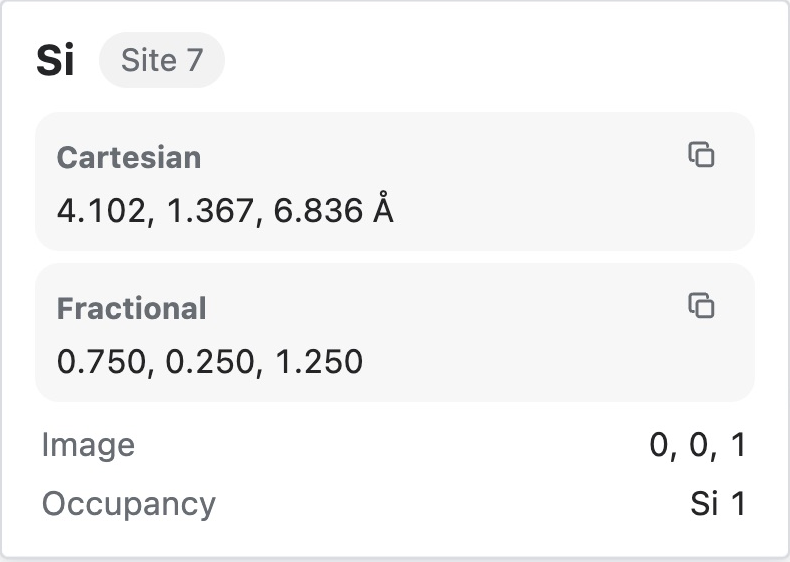
\includegraphics[width=79mm]{publication-assets/crop-4ce96785f91c44d963be.png}
\caption{Online中Site 7周期映像的原子信息卡局部。分数坐标和映像偏移应一起阅读；该原子仍属于模型的第7个位点。\ui{Occupancy}中的Si 1表示该位点由硅完全占据。}
\label{fig:si-periodic-image-inspection}
\end{figure}

\subsection{显示更多晶胞}

有时，一个晶胞不足以看清晶体中的连续连接。在三维视图自己的工具栏打开查看器设置，找到 \ui{Repeat cell}，将 $a$、$b$、$c$ 三个方向分别设为\mbox{2、2、1}。视图会显示更多周期映像，从而更容易辨认空间排列。观察完成后，可使用恢复按钮回到 $1\times1\times1$。

这项设置只控制显示重复范围。它不会把项目中的 8 原子结构变成一个用于计算的更大模型。需要模拟局域缺陷或降低周期映像之间的相互影响时，应使用后面的\ui{构建超胞}命令。两者虽然都可能让屏幕上出现更多原子，改变的对象却不同。

\subsection{调整表示方式}

球棍表示适合辨认连接关系，较大的原子半径适合观察原子占据的空间。查看器设置中可选择元素配色、原子半径方式和原子比例，控制化学键、晶胞边框、配位多面体等对象的显示。制作讲义或报告时，先确定需要说明的问题，再选择表示方式；同一张图同时打开所有辅助对象，往往会遮住需要观察的局部结构。

晶体中的化学键常由邻近关系分析得到。改变成键策略后，显示的键可能发生变化，而原子的实际位置没有变化。对于具有明确拓扑的分子，应优先使用源文件中的连接关系；对于晶体，应结合配位环境理解显示结果。单凭一根显示出来的连线，不能推断该体系已经完成了电子结构分析。

\section{精确编辑原子}

\subsection{形成合适的选择}

单击可以选择原子，按住 Shift 或 Ctrl 再单击可以加入或移出当前选择。双击可选择相连结构。原子较多时，按 B 后拖动进行框选，按 L 后拖动进行套索选择。按 Cmd/Ctrl+A 可全选，按 Esc 退出当前工具或清除选择。

选择并不一定等于屏幕上被圈住的所有球。例如，周期显示可能包含同一个底层位点的不同映像。编辑前应查看选择数量和位点序号，尤其是在显示重复范围大于一个晶胞时。需要多次使用同一组位点，可将选择保存为选择集，之后从\ui{选择集}菜单重新调用。

\begin{notebox}{为什么 sites 与 atoms 不同}
查看器摘要中的 \ui{sites} 表示模型的独立位点数，\ui{atoms} 则包含用于显示边界和周期连接的原子映像。核对超胞倍数、元素计数或缺陷数量时，应以模型位点数为准。一个 8 位点硅晶胞可以显示多于 8 个原子球；建立 $2\times2\times2$ 超胞后，应检查 64 个位点，而不是要求屏幕上的原子球数量恰好等于 64。
\end{notebox}

\begin{figure}[htbp]
\centering
\begin{tikzpicture}[x=1mm,y=1mm,font=\sffamily\small]
  \node[text=brand] at (21,42) {模型：2 个独立位点};
  \node[text=brand] at (85,42) {视图：位点与映像};
  \fill[paleblue] (5,0) rectangle (37,32);
  \fill[paleblue] (69,0) rectangle (101,32);
  \draw[teal,line width=.75pt] (5,0) rectangle (37,32);
  \draw[teal,line width=.75pt] (69,0) rectangle (101,32);
  \fill[brand] (5,0) circle (2.3);
  \fill[teal] (21,16) circle (2.3);
  \node[text=white,font=\sffamily\scriptsize] at (5,0) {A};
  \node[text=white,font=\sffamily\scriptsize] at (21,16) {B};
  \fill[brand] (69,0) circle (2.3);
  \fill[teal] (85,16) circle (2.3);
  \node[text=white,font=\sffamily\scriptsize] at (69,0) {A};
  \node[text=white,font=\sffamily\scriptsize] at (85,16) {B};
  \foreach \x/\y in {101/0,69/32,101/32} {
    \draw[fill=white,draw=brand,line width=.8pt] (\x,\y) circle (2.3);
    \node[text=brand,font=\sffamily\scriptsize] at (\x,\y) {A};
  }
  \draw[->,>=stealth,teal,line width=.75pt] (43,16) -- (61,16);
  \node[text=brand,font=\sffamily\footnotesize] at (52,23) {周期显示};
  \node[text=ink,font=\sffamily\footnotesize,align=center] at (21,-8) {只保存 A、B 两个位点};
  \node[text=ink,font=\sffamily\footnotesize,align=center] at (85,-8) {空心圆是 A 的边界映像};
\end{tikzpicture}
\caption{独立位点与边界映像（二维示意）。同一位点 A 可以出现在多个周期边界上，绘制更多原子球并没有增加模型中的独立位点。}
\label{fig:periodic-sites}
\end{figure}


对需要严格指定顺序的几何操作，建议先清除选择，再逐个点选。两原子给出距离；三个原子定义以第二个原子为顶点的角；四个原子依次定义二面角。顺序改变，几何量的含义也可能改变。

\subsection{直接拖动与数值编辑}

选好原子后，按 G 再拖动可移动选择，按 R 再拖动可旋转选择；变换过程中按 X、Y 或 Z 可以约束方向。直接拖动适合安排大致构型。若需要确定的位移、转角或键长，应打开对应参数命令，用数值完成最后一步。

\ui{平移原子}输入的是位移向量，而\ui{移动原子}输入的是新的坐标。将一个原子从 $(1,0,0)$ 移到 $(2,0,0)$，可以给它平移 $(1,0,0)$，也可以把新坐标设为 $(2,0,0)$。在晶体中，两类命令还允许使用相应的分数或笛卡尔表示，输入前应检查坐标选项。

\ui{旋转原子}需要转轴、角度和锚点。角度以度为单位；锚点是转轴经过的位置。若希望一个片段绕自己的连接位点转动，应把锚点放在连接位点附近，而不是沿用与片段相距很远的原点。这样，预览中的运动更符合预期。

% SCREENSHOT: 一个局部分子选择及精确平移/旋转参数窗口，画面中保留选择高亮。

\section{提交结构修改}

大多数会改变结构的参数对话框都提供\ui{预览}、\ui{应用}和\ui{取消}。预览用于检查参数的几何效果；应用将修改写入当前文档的编辑状态；保存再将该状态写回项目。第一次使用新命令时，可以先走一次“预览—取消”，确认模型能恢复，再重新执行并应用。

\begin{steps}
  \item 打开需要的建模命令，核对当前选择与参数单位。
  \item 输入参数后单击\ui{预览}。转动或缩放视图，检查模型中发生变化的部位。
  \item 若结果合适，单击\ui{应用}；若不合适，修改参数重新预览，或单击\ui{取消}恢复原视图。
  \item 应用后检查原子数量、晶胞或几何值。可用 Cmd/Ctrl+Z 撤销，用 Shift+Cmd/Ctrl+Z 重做。
  \item 完成一段有意义的工作后保存项目，并为模型保留清楚的名称。
\end{steps}

\ui{历史}区域中的\ui{重置}恢复打开当前文档或最近保存时的结构。它与重新居中相机的按钮不同。保存后，最近保存的模型会成为新的编辑基准，当前撤销历史随之清空；如果希望长期比较两套模型，应保留两个有明确名称的项目结构，而不要只依赖撤销记录。

纯分析命令不一定产生新的结构预览，结果的显示方式也因命令而异。\ui{分子诊断}按规则检查当前分子的价态、近距离接触和键长，不改变结构；当前图形界面完成后显示\ui{Molecule diagnostics completed.}，没有展开逐项问题表。这个提示表示命令已经结束，结构是否合适还要结合组成、连接和几何读数判断。具体检查方法见本章\ref{sec:molecule-manual-check}节；完整MATLAB中的配套脚本另保留诊断数据。

\section{示例：硅超胞与一个空位}

\subsection{把晶胞扩大为超胞}
\index{Chaobao@超胞}

超胞把基本晶胞沿选定方向复制，并把复制得到的全部原子作为新模型的一部分。对于对角重复 $(n_x,n_y,n_z)$，原子数和体积均扩大 $n_xn_yn_z$ 倍。本例从 8 位点硅晶胞建立 $2\times2\times2$ 超胞，因而模型应包含 64 个独立位点。这个数量由输入文件和重复倍数确定，可用来检查操作。

\begin{steps}
  \item 回到由 \file{Si.poscar} 导入的 \file{Si} 文档，将显示重复恢复为 $1\times1\times1$，避免把显示映像与模型原子混淆。
  \item 在顶部\ui{晶体建模}的\ui{晶体与晶胞}区域打开\ui{超胞与晶格}，选择\ui{构建超胞}。
  \item 在\ui{超胞倍率或变换矩阵}中核对默认的 \literalinput{2 2 2}，单击\ui{预览}。从晶胞边框观察三个方向的扩大；窗口下方会提示预览已显示。
  \item 先单击\ui{取消}，确认回到原晶胞，摘要仍为8个位点。再次打开同一命令，核对相同参数并单击\ui{应用}。
  \item 检查模型有64个硅位点，三个晶格矢量长度分别为原来的两倍。本次实机显示64 sites、166 atoms；核对扩胞倍数时看前者。如需长期保留无缺陷超胞，可以在继续创建空位前另存一个项目副本。
\end{steps}

一般超胞由一个整数矩阵 $S$ 定义。矩阵的每一行说明一条新晶格矢量由原来的三条矢量怎样组合。例如，第一行为 $(2,1,0)$，就表示 $\mathbf a'=2\mathbf a+\mathbf b$。在本书的行向量约定下，晶格、体积和位点数满足
\begin{equation}
 A'=SA,\qquad V'=|\det S|V,\qquad N'=|\det S|N.
 \label{eq:supercell-count-volume}
\end{equation}
$S$ 中的数必须是整数，且行列式不能为零。$|\det S|$ 是新旧晶胞的体积比，也是独立位点数的倍数；$N$ 始终数模型位点，不数边界上额外绘出的原子映像。对于三个重复数，$S=\operatorname{diag}(n_a,n_b,n_c)$，式\eqref{eq:supercell-count-volume}就回到三个重复数相乘的规则。上面的实机练习取 $S=2I$，所以 $|\det S|=8$，8个位点变为64个。

下面用一个非对角矩阵作代数检查：
\[
 S=\begin{bmatrix}2&1&0\\0&1&0\\0&0&1\end{bmatrix},\qquad
 \begin{cases}
 \mathbf a'=2\mathbf a+\mathbf b,\\
 \mathbf b'=\mathbf b,\quad \mathbf c'=\mathbf c.
 \end{cases}
\]
其行列式为2。若原模型含8个位点，新模型应含16个位点，体积是原来的两倍；新外框可以倾斜，周期材料本身的局部排列仍来自原结构的复制。这与通过应变拉伸原子间距有区别：超胞选择更大的重复单元，不把每条原子间连接都拉长两倍。

在\ui{超胞倍率或变换矩阵}中，可以填写三个重复整数，也可以填写完整的 $3\times3$ 矩阵。使用一般矩阵前先写出三条新基矢，再检查行列式、预览外框和应用后的位点数，便不容易把“重新定向”和“增加了多少原子”混为一谈。输入\literalinput{1 1 1}时，矩阵为 $I$，模型不扩大；本工具仍会把等价坐标归入单位晶胞，适合将落在胞外的代表位置整理到同一胞中查看。


\begin{figure}[!htb]
\centering
% 原图3024×1758；完整窗口(670,585,2355,1455)，1685×870；122mm约351ppi。
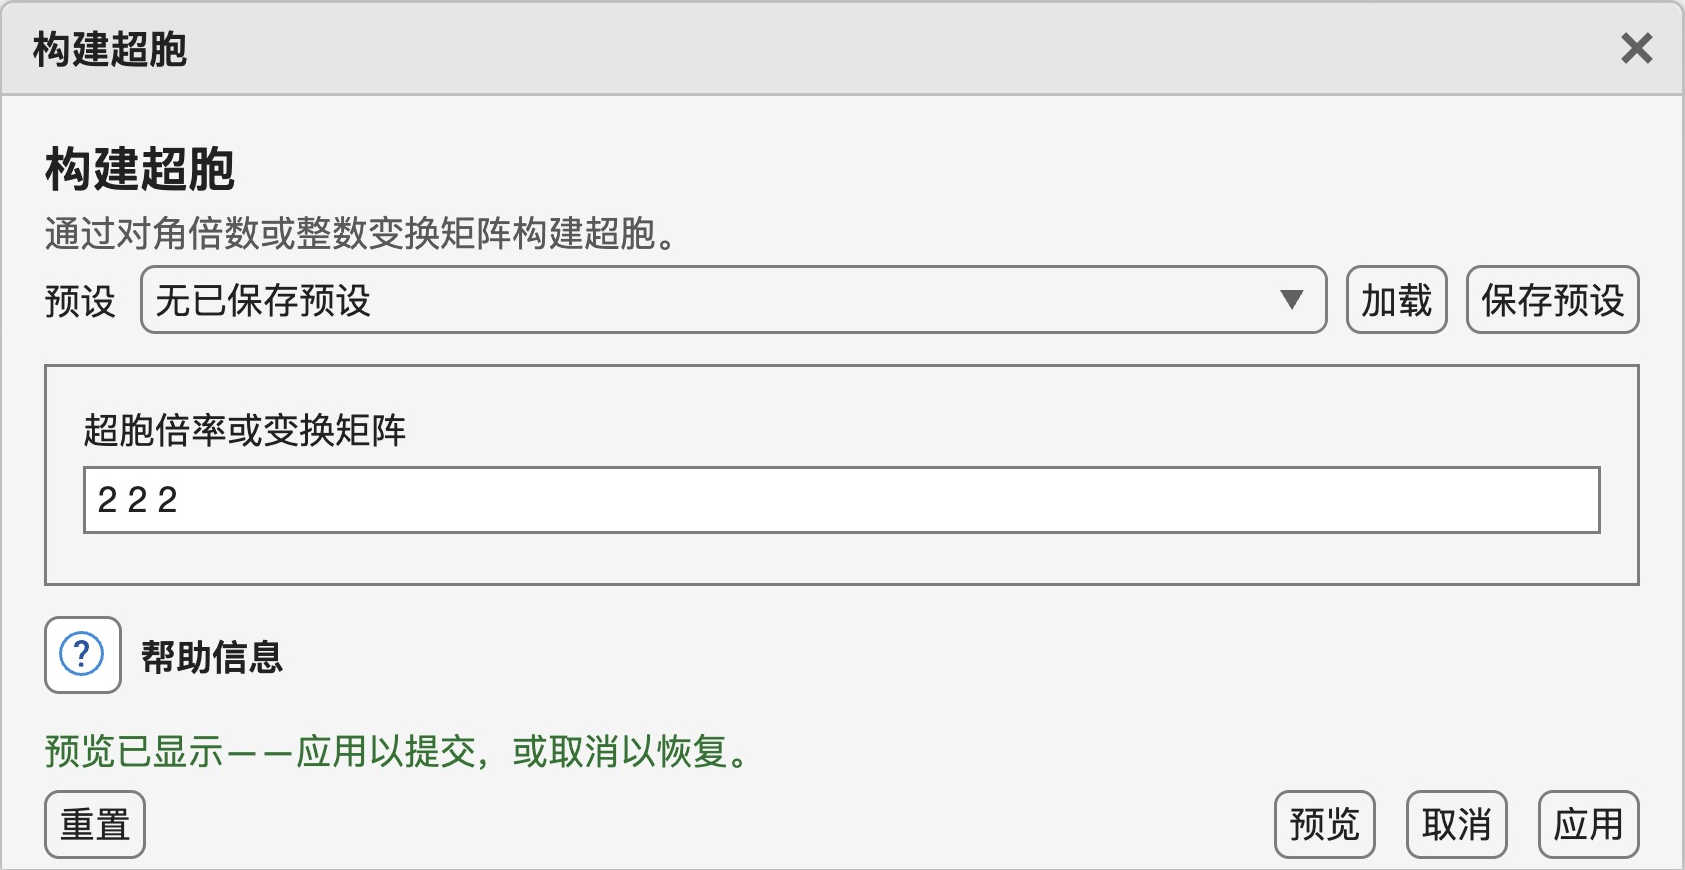
\includegraphics[width=\linewidth]{publication-assets/crop-0ff9d4164c5629316893.png}
\caption{构建超胞的参数与预览状态。\literalinput{2 2 2}表示三个方向分别重复两次；本例先取消一次预览，再重新打开并应用。}
\label{fig:si-supercell-preview}
\end{figure}

\begin{figure}[!htb]
\centering
\begin{minipage}[b]{78mm}
% 原图3024×1758；完整模型(875,365,2155,1615)，1280×1250；78mm约417ppi。
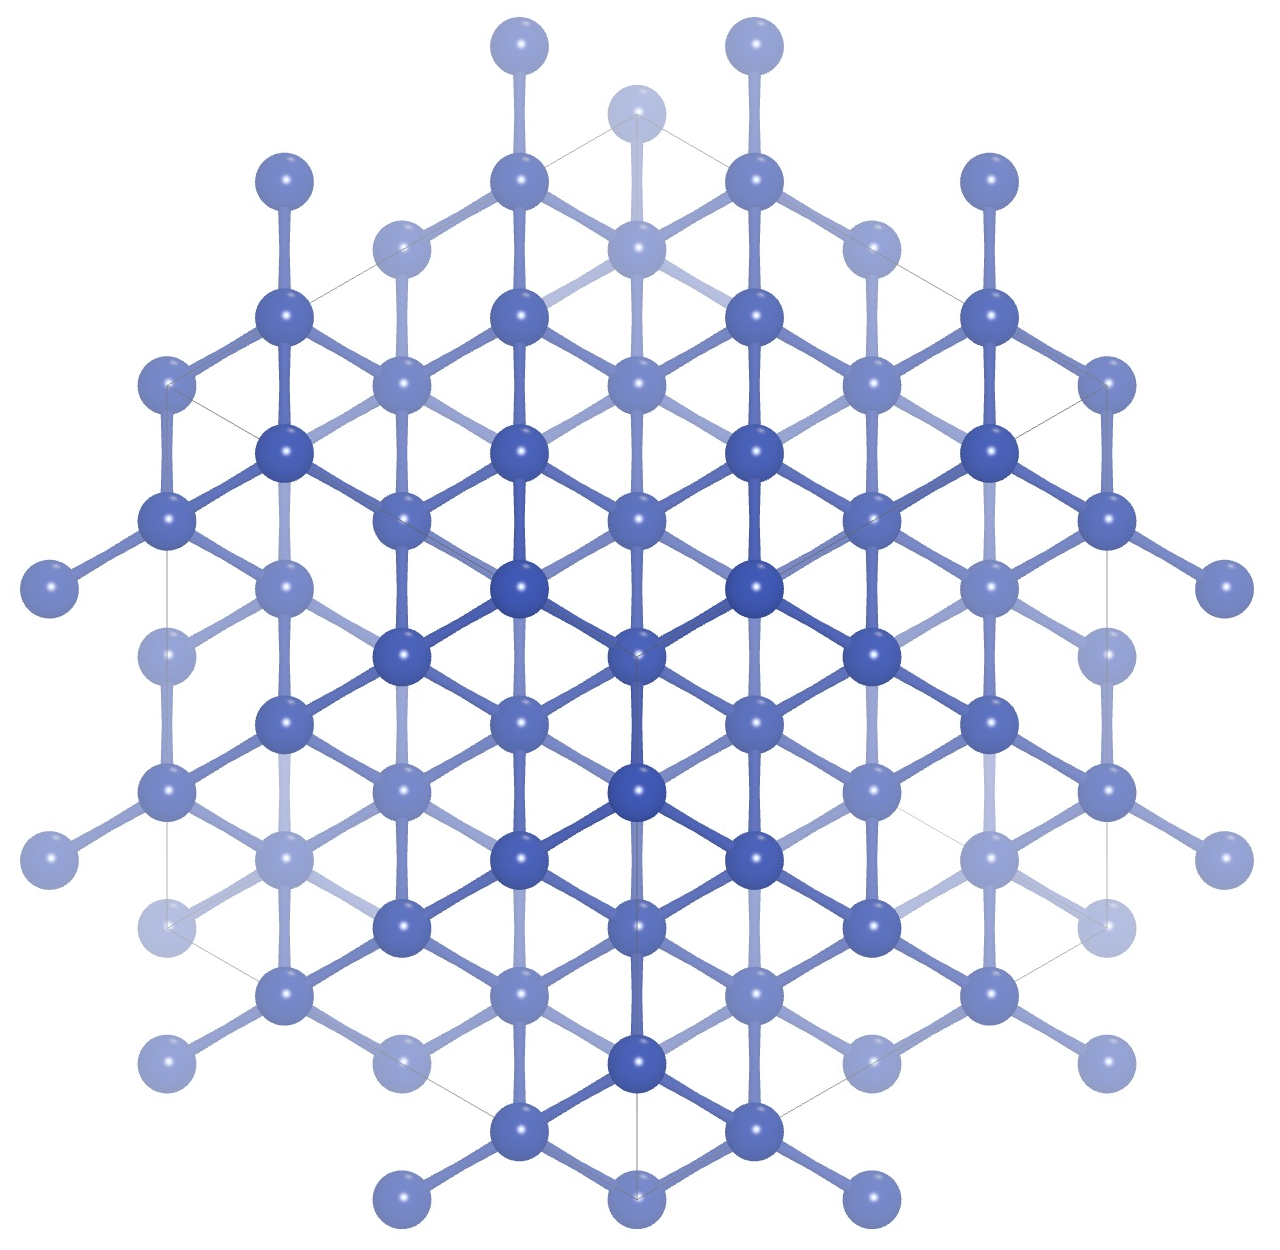
\includegraphics[width=\linewidth]{publication-assets/crop-0469f894473f746988e3.png}
\end{minipage}\hfill
\begin{minipage}[b]{42mm}
% 同图独立摘要(45,330,465,560)，420×230；42mm约254ppi。
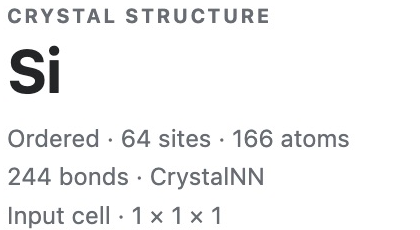
\includegraphics[width=\linewidth]{publication-assets/crop-c0154093dad09f77a9a2.png}
\end{minipage}
\caption{Online中应用后的硅超胞，分别呈现完整模型与摘要局部。64 sites是模型独立位点数，166 atoms包含边界映像；\ui{Input cell $1\times1\times1$}是对新超胞的显示范围。}
\label{fig:si-supercell-result}
\end{figure}

\subsection{创建并检查空位}
\index{Kongwei@空位}

空位表示从晶格中的一个位点移去原子。建立空位前先扩大晶胞，可以减小相邻周期映像之间的距离过近所带来的影响；具体需要多大超胞，应结合后续计算的收敛检查决定。本例只练习构建，不计算缺陷形成能。

\begin{steps}
  \item 确认当前活动文档仍是刚建立的64位点 \file{Si} 超胞。本例移去原子序号1。
  \item 在\ui{晶体建模}的\ui{晶体材料}区域打开\ui{缺陷与合金}，依次选择\ui{创建点缺陷 → 空位}。在参数窗口核对\ui{缺陷类型}为\ui{空位}，\ui{原子序号（从 1 开始）}输入\file{1}。
  \item 核对类型和序号后单击\ui{应用}。转动视图，观察移去原子后邻近位置的连接。
  \item 检查位点数由64变为63，晶胞仍是所建立的超胞。本次摘要为63 sites、162 atoms；显示映像减少的数量不必等于移去的独立位点数。
  \item 使用\ui{另存为}保存为\file{Si-vacancy-tutorial.ks}，保留原来的\file{Si-introduction.ks}。保存后检查标题中的未保存星号已消失。
\end{steps}

\begin{figure}[!htb]
\centering
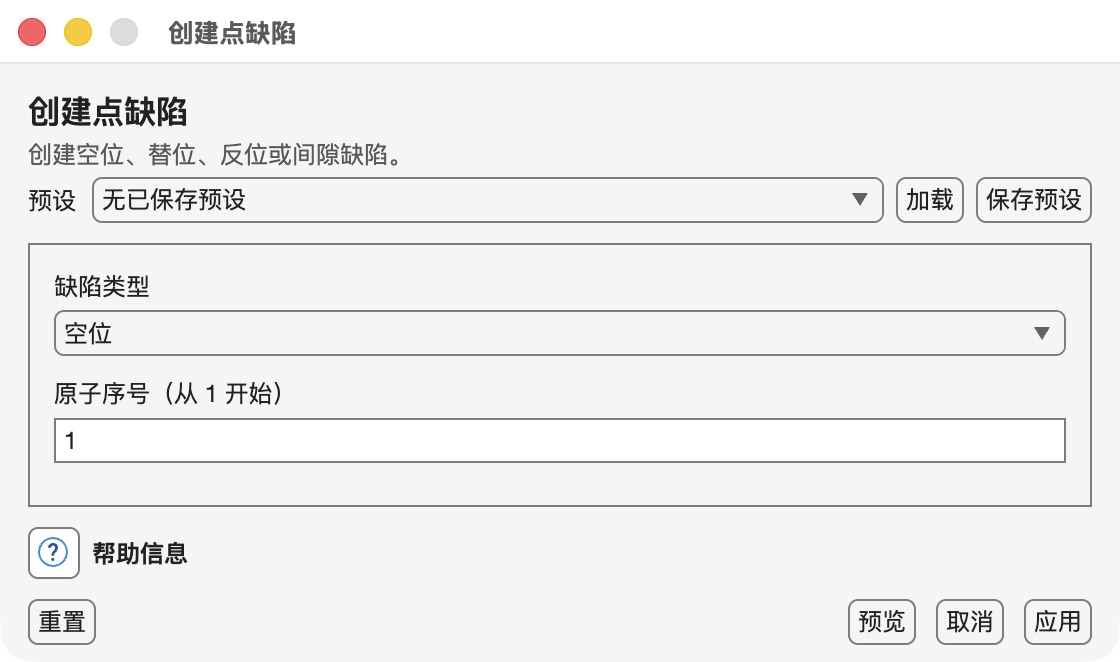
\includegraphics[width=113.7mm]{publication-assets/crop-601f9ce2a238baeb7b2e.png}
\caption{创建硅空位的参数。缺陷类型为\ui{空位}，原子序号为1；应用后按正文检查独立位点由64减为63。}
\label{fig:si-vacancy-settings-result}
\end{figure}

随书的\file{Si-vacancy-tutorial.ks}来自这次实际另存，包含原来的\file{silicon}对照结构和完成空位编辑的\file{Si}结构。需要无缺陷超胞作对照时，可从\file{Si.poscar}按上述步骤重新建立64位点模型，并在创建空位前另存。

晶体原子编辑中的对称性处理会影响等价位置。如果目的是局域缺陷，应明确自己需要的是单个位点变化，还是整组等价位点的变化。\ui{创建点缺陷}提供了直接表达空位、替位、间隙和反位的入口；不要仅凭屏幕上消失了一个球就结束检查。

\section{示例：从芳香环建立苯和吡啶}
\index{Fangxiang fenzi@芳香分子}

\subsection{建立苯分子的骨架}

分子草绘可以在三维视图中逐个放置原子，也可以用环和片段快速建立骨架。按 S 进入草绘后，单击空白处放置独立原子，从已有原子拖动可添加相连原子，拖向另一已有原子可建立连接。草绘栏用于选择元素、键级和环。

本例先通过参数命令建立规则六元环，便于理解芳香性和加氢的作用。

\begin{steps}
  \item 选择\ui{主页 → 结构 → 新建结构 → 空白分子结构}，激活新文档，在\ui{分子建模}中打开\ui{绘制环}。
  \item 环尺寸设为 6，元素为 C，边长为 $1.4\,\text{\AA}$，启用芳香环。中心的三个数值框分别填 0、0、0；法向的三个数值框分别填 0、0、1。
  \item 保持不连接到其他原子，预览并应用。此时得到碳骨架，尚需补足氢。
  \item 按 Cmd/Ctrl+A 选中六个环原子，运行\ui{添加氢}。检查应形成苯的组成 $\mathrm{C_6H_6}$。
  \item 运行\ui{分子诊断}，关闭完成提示。旋转视图，检查六元环、每个碳相连的氢和局部距离，再保存模型，命名为\file{Benzene}。
\end{steps}

芳香环的连接信息与普通单键环不同。仅把六个碳摆成六边形，或仅让显示的键看起来相同，都不能替代芳香键和原子化学性质的设置。检查模型时，应同时观察分子组成、键级与芳香标记。

补氢后还应转到侧面检查整个分子。环骨架共面，并不表示自动放置的氢已经落在环平面内。随书的\file{benzene.json}保留本例补氢后的初始状态，\mbox{\file{benzene-optimized.json}}保留通用分子模型优化后的状态，便于对照；后者仍是建模参考结构。需要单独交换这些芳香分子时，可使用原生 JSON 保存化学属性与芳香键，并在重新导入后核对连接。

\subsection{把一个碳改为氮}

先保存当前苯模型，再选择\ui{主页 → 结构 → 从文件导入结构…}，再次导入随书\file{benzene.json}，打开新导入的结构，用它练习吡啶。这样可以保留原来的苯作为对照。为使加氢过程清楚，先移除氢，再替换环上的一个碳。

\begin{steps}
  \item 在新导入的结构中全选并运行\ui{删除氢}，随后选择一个环碳，打开\ui{原子化学属性}。
  \item 将元素改为 N，形式电荷为 0，杂化设为 \file{sp2}，保持芳香原子选项。
\end{steps}

% Online实机吡啶示例；由主控插入第7章适当位置。
% 仅以LaTeX矩形裁切原JPEG，不修改、拼接或重绘像素。
\begin{figure}[H]
\centering
% 原图3024×1758；参数范围(710,735,2315,1585)，1605×850，122mm约334ppi。
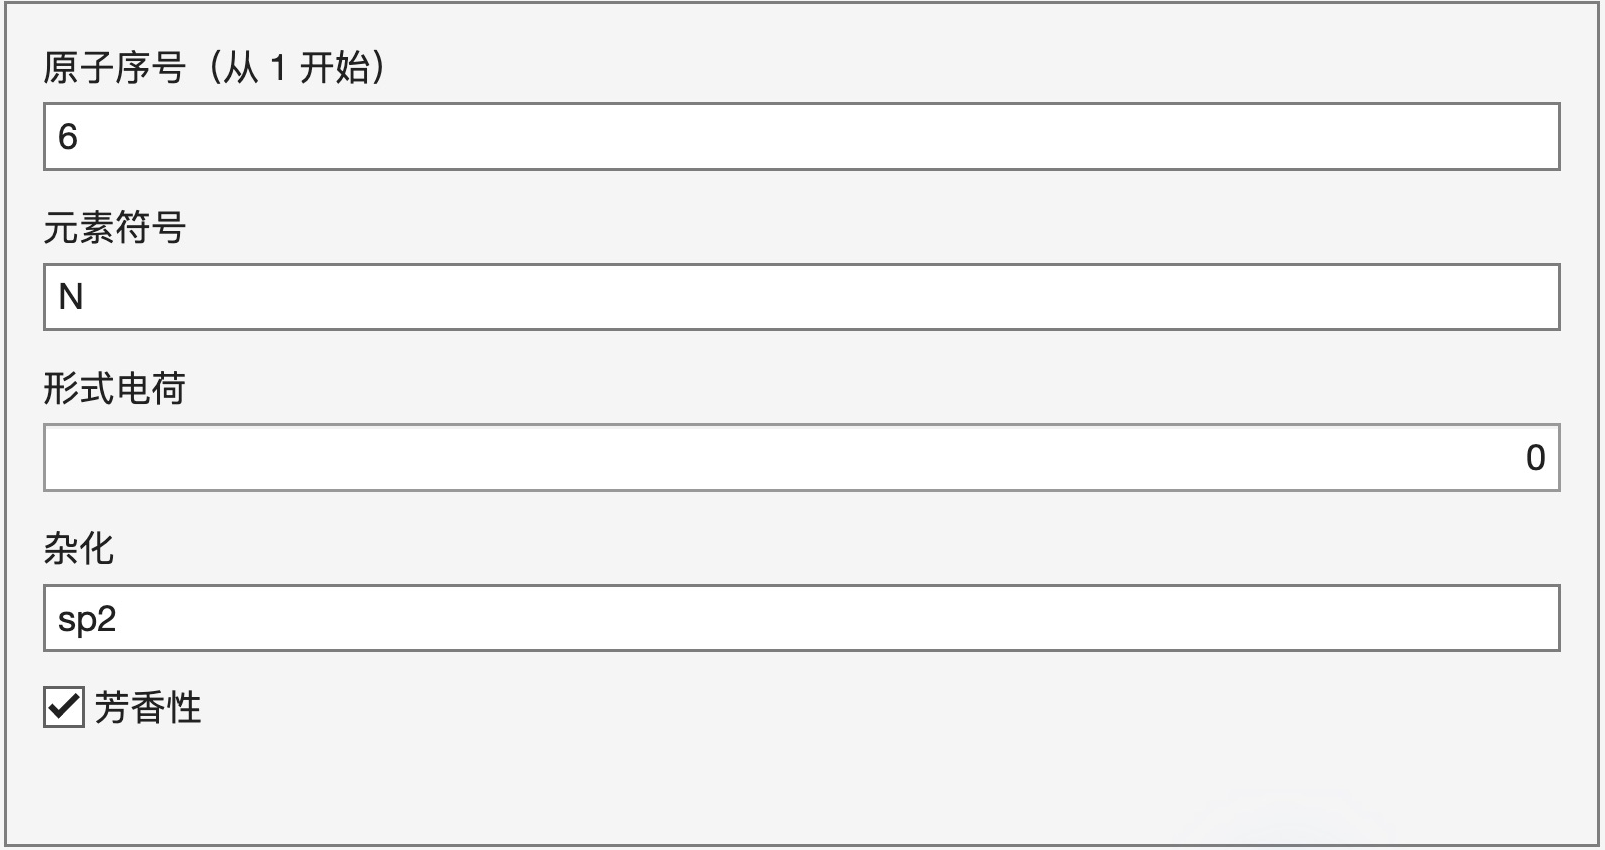
\includegraphics[width=\linewidth]{publication-assets/crop-f99354db0f163eccfd81.png}
\par\vspace{2mm}
% 同一原图的独立预览提示范围(700,1615,1520,1670)，820×55；排除右侧指针。
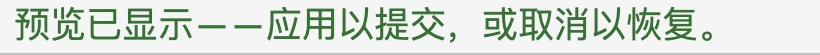
\includegraphics[width=80mm]{publication-assets/crop-8ce96edd826deccee006.png}
\caption{Online中把环上第6个原子替换为氮的实际参数：元素为N，形式电荷为0，杂化为\ui{sp2}，勾选\ui{芳香性}。下方为同一次操作的预览提示；此时仍需单击应用提交。}
\label{fig:pyridine-chemistry}
\end{figure}


\begin{steps}[resume]
  \item 应用后全选环原子并\ui{添加氢}，检查组成应为 $\mathrm{C_5H_5N}$，并检查氮附近的连接。
  \item 运行\ui{分子诊断}，关闭完成提示后，回到视图比较苯与吡啶的组成、环连接和氮附近的氢数。可导入随书\file{pyridine.json}，对照完整的中性吡啶模型。
\end{steps}

形式电荷、杂化提示与元素共同影响连接关系的解释。若替换元素后继续沿用原先全部氢原子，可能得到与预期不同的价态。对于这类修改，先处理骨架再补氢，通常更容易检查。

中性吡啶有 42 个电子，本例采用单重态。当前版本从含奇数电子的骨架继续加氢时，可能保留骨架的自旋多重度，导致再次读取文件时提示电荷与自旋不匹配。随书的\file{pyridine.json}已校正为电荷 0、多重度 1；需要继续计算时，可以从这份文件开始。

图\ref{fig:pyridine-chemistry}记录了本次将第6号环原子改为氮的参数；图\ref{fig:pyridine-built-model}可用于核对补氢后的六元环和五个氢原子。

% 吡啶应用和补氢后的结果，接在读者检查步骤之后。
\begin{figure}[H]
\centering
% 原图3024×1758；几何范围(900,370,2120,1680)，1220×1310；70mm约443ppi。
% 不包含摘要；当前会话保留骨架多重度的现象由第7章正文另行说明。
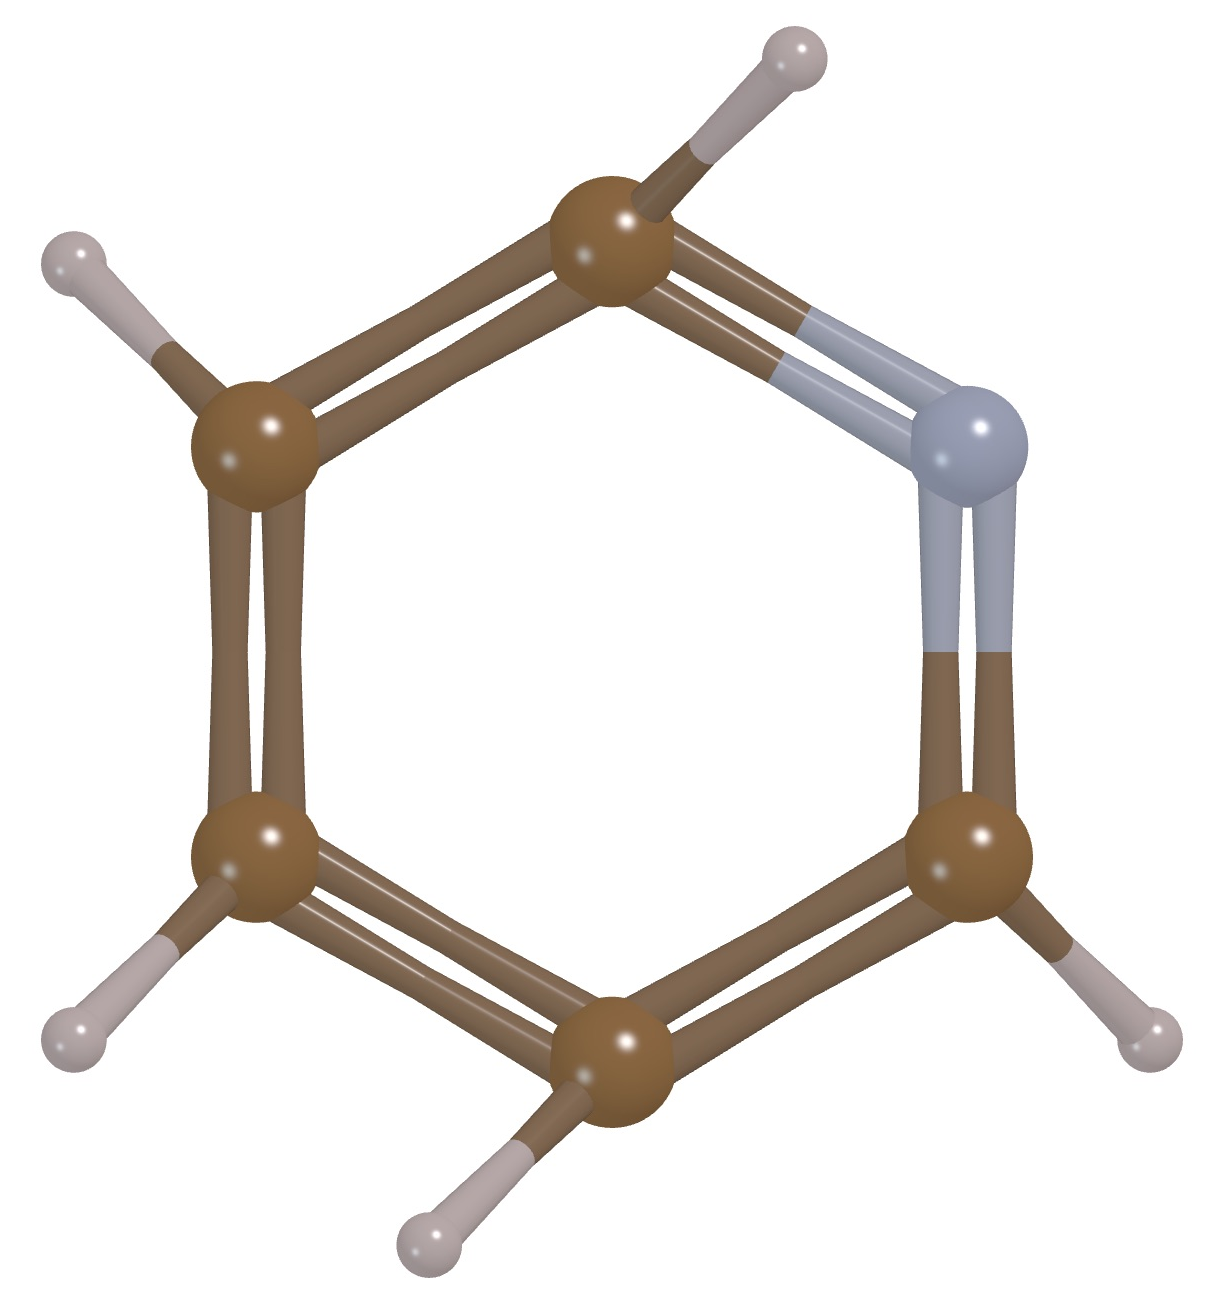
\includegraphics[width=70mm]{publication-assets/crop-60c8057a2bb7c31f0fd8.png}
\caption{Online中完成元素替换并对六个环原子补氢后的实际几何：五个碳、一个氮和五个氢，共11个原子、11条连接。此图未经过几何优化；继续计算时，使用随书\file{pyridine.json}中已修正的中性单重态参考结构。}
\label{fig:pyridine-built-model}
\end{figure}


% SCREENSHOT: 尚需苯芳香环绘制参数与实际环预览；吡啶属性和补氢几何已由fig:pyridine-chemistry及fig:pyridine-built-model覆盖。分子诊断实机仅显示完成提示，不要求或暗示存在详细诊断表。

\section{示例：调整乙醇构象}
\index{Fenzi jihe@分子几何}

\subsection{建立连接清楚的初始分子}

乙醇的重原子骨架是 C--C--O。先选择\ui{主页 → 结构 → 新建结构 → 空白分子结构}，打开新文档，再依次草绘三个原子并添加氢；也可以通过添加原子和建键命令完成。为了使输入便于核对，本例使用以下初始坐标，长度单位为 \AA。

\begin{table}[htbp]
\centering
\caption{乙醇骨架的练习输入。共线坐标只用于开始几何编辑。}
\begin{tabularx}{\linewidth}{lX}
\toprule
原子与序号 & 输入与连接 \\
\midrule
1：C & 坐标 $(0,0,0)$；作为第一个独立原子。\\
2：C & 坐标 $(1.52,0,0)$；与原子 1 以单键连接。\\
3：O & 坐标 $(2.95,0,0)$；与原子 2 以单键连接。\\
\bottomrule
\end{tabularx}
\end{table}

当草绘命令启用了\ui{使用力场理想键长}时，工具会按连接方向采用理想键长。需要严格使用表中的练习坐标时，关闭这一选项。骨架建立后补氢，检查组成应为 $\mathrm{C_2H_6O}$。这一初始构型还没有经过几何整理，不宜将其中的共线骨架当成乙醇的稳定构型。

\subsection{设置几何量}
\index{Juli@距离测量}
\index{Jianjiao@键角}
\index{Ermianjiao@二面角}

需要读取距离时，在三维视图工具栏的\ui{Measurements}中选择\ui{Atom-to-atom distance}，再依次单击原子1、2。要修改距离，打开顶部\ui{设置距离}，在原子序号中填\literalinput{1 2}，把目标设为$1.52\,\text{\AA}$。接着打开\ui{设置键角}，原子序号填\literalinput{1 2 3}，目标填$109.5^\circ$。本例的距离、键角和二面角操作均选择\ui{子树}移动范围，使相连的原子一起调整。

\ui{原子}范围只移动局部原子；\ui{子树}沿连接关系移动一侧；\ui{片段}用于对一个连接片段整体调整。改变键角时，如果只移动一个重原子而没有带动其相连氢，附近几何可能变差。预览时应把整个分子纳入观察，而不要只看目标角的数值。

\begin{steps}
  \item 对 C--C--O 骨架设置需要的距离和角度，每次应用后重新测量一次。
  \item 调整视图，按需要依次选择四个相连原子，例如 C--C--O--H。确认最后一个是与 O 相连的氢。
  \item 在\ui{设置二面角}中输入一个便于比较的角度，例如 $60^\circ$，使用预览观察末端片段的转动。
  \item 换用另一二面角后再次观察，并用撤销返回前一构型。通过这一对比理解构象变化，而不是把某个输入角度直接解释为能量最低构象。
\end{steps}

\subsection{在查看器中核对键角}

几何编辑后的数值，可在三维视图自己的测量卡片中读取。顶部\ui{几何编辑 → 测量几何}是另一个命令；当前图形界面完成后只显示\ui{Geometry measurement completed.}，不在提示框中列出数值。需要检查角度时，按下面的查看器步骤操作。

图\ref{fig:ethanol-angle-parameters}与图\ref{fig:ethanol-angle-measured}记录了一次实际练习。为便于选择原子，这次另从随书\mbox{\file{ethanol-optimized.json}}导入副本，再修改指定角度；它与前面从共线骨架逐步建立分子的过程采用不同的起点。

\begin{steps}
  \item 导入\mbox{\file{ethanol-optimized.json}}，打开副本的分子文档，保留原文件作为参考。
  \item 在\ui{设置键角}中填写原子\literalinput{1 2 3}、目标$109.5^\circ$与\file{subtree}移动范围，先预览，再应用。此处只是练习几何编辑，不是在重新优化分子。
\end{steps}

% Online实际乙醇设置/测量；只以LaTeX裁切原生JPEG，不修改像素。
\begin{figure}[H]
\centering
% 原图3024×1758；(710,820,2310,1400)，1600×580，122mm约333ppi。
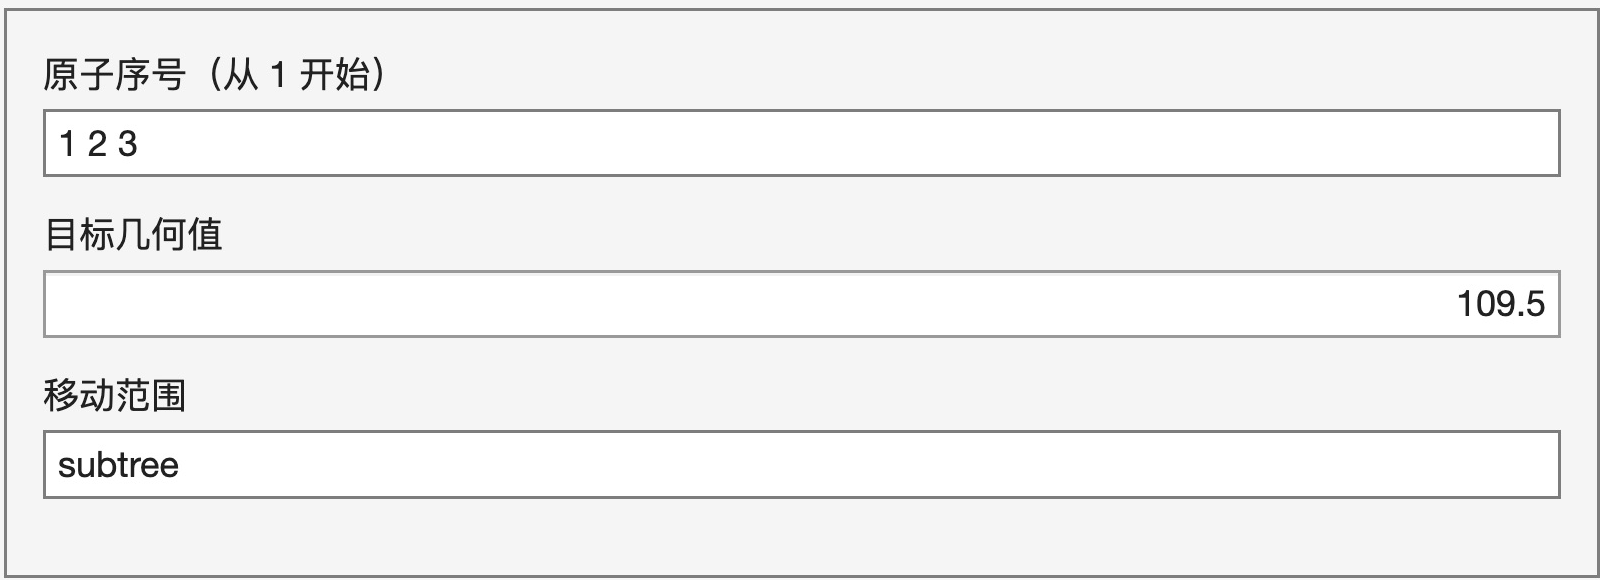
\includegraphics[width=\linewidth]{publication-assets/crop-0483f84ce4963946e315.png}
\par\vspace{2mm}
% 独立状态局部(710,1425,1520,1482)，810×57；去掉上方指针及下方按钮边缘。

\includegraphics[width=80mm]{publication-assets/crop-17309e4ada4dd6ce532b.png}
\caption{Online中重新设置乙醇键角的实际参数。按顺序输入原子\literalinput{1 2 3}，目标为$109.5^\circ$，移动范围为\file{subtree}；下方提示预览已显示，仍需应用提交。}
\label{fig:ethanol-angle-parameters}
\end{figure}


\begin{steps}[resume]
  \item 关闭参数窗口，在三维视图右侧工具栏找到尺形的\ui{Measurements}按钮，选择\ui{Bond angle}。进入测量后，按新的顺序重新点选原子。
  \item 依次单击1号C、2号C、3号O，第二个原子是角的顶点。本次视图中1号C在上方，2号C在中间，O为红色。完成第三次点选后，左侧测量卡片显示角度和原子路径，模型中出现两条角边与圆弧。
  \item 核对卡片为$109.500^\circ$，路径为\ui{\#1 C}、\ui{\#2 C}、\ui{\#3 O}。记下测量值与原子顺序，关闭结果卡片，再保存修改后的副本。
\end{steps}

这个读数确认刚才的几何编辑已经得到指定角度，不代表乙醇的平衡键角。需要比较优化前后时，应对两份分别保存的模型采用同一原子顺序测量，并记录各自实际读数。

% 乙醇实际测量结果，接在查看器点选与读数步骤之后。
\begin{figure}[H]
\centering
\begin{minipage}[t]{62mm}
\vspace{0pt}
% 测量卡片(55,328,845,1717)，790×1389；62mm约324ppi。
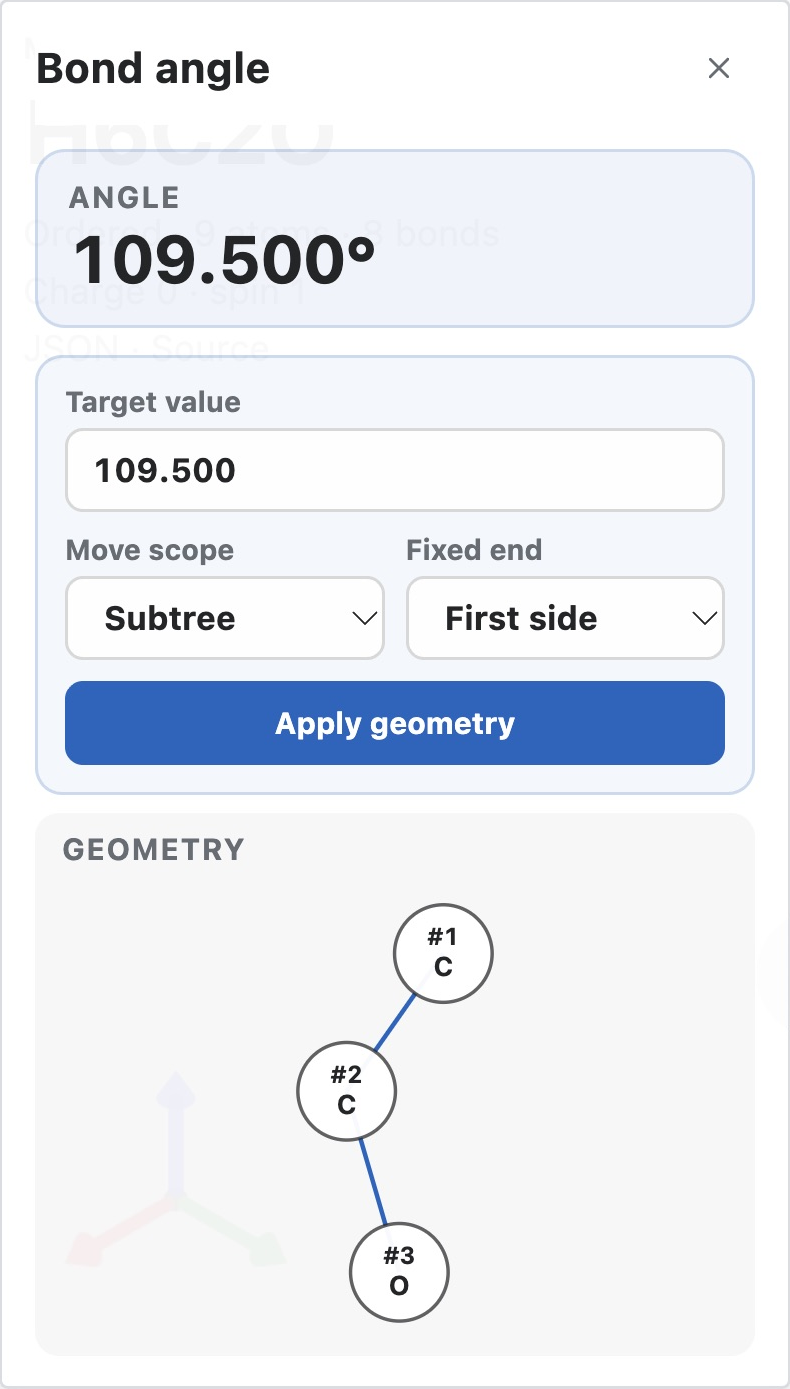
\includegraphics[width=\linewidth]{publication-assets/crop-cdb0f92bdcdbb307f144.png}
\end{minipage}\hfill
\begin{minipage}[t]{58mm}
\vspace{0pt}
% 三重原子和实际角线(850,400,2000,1650)，1150×1250；58mm约504ppi。
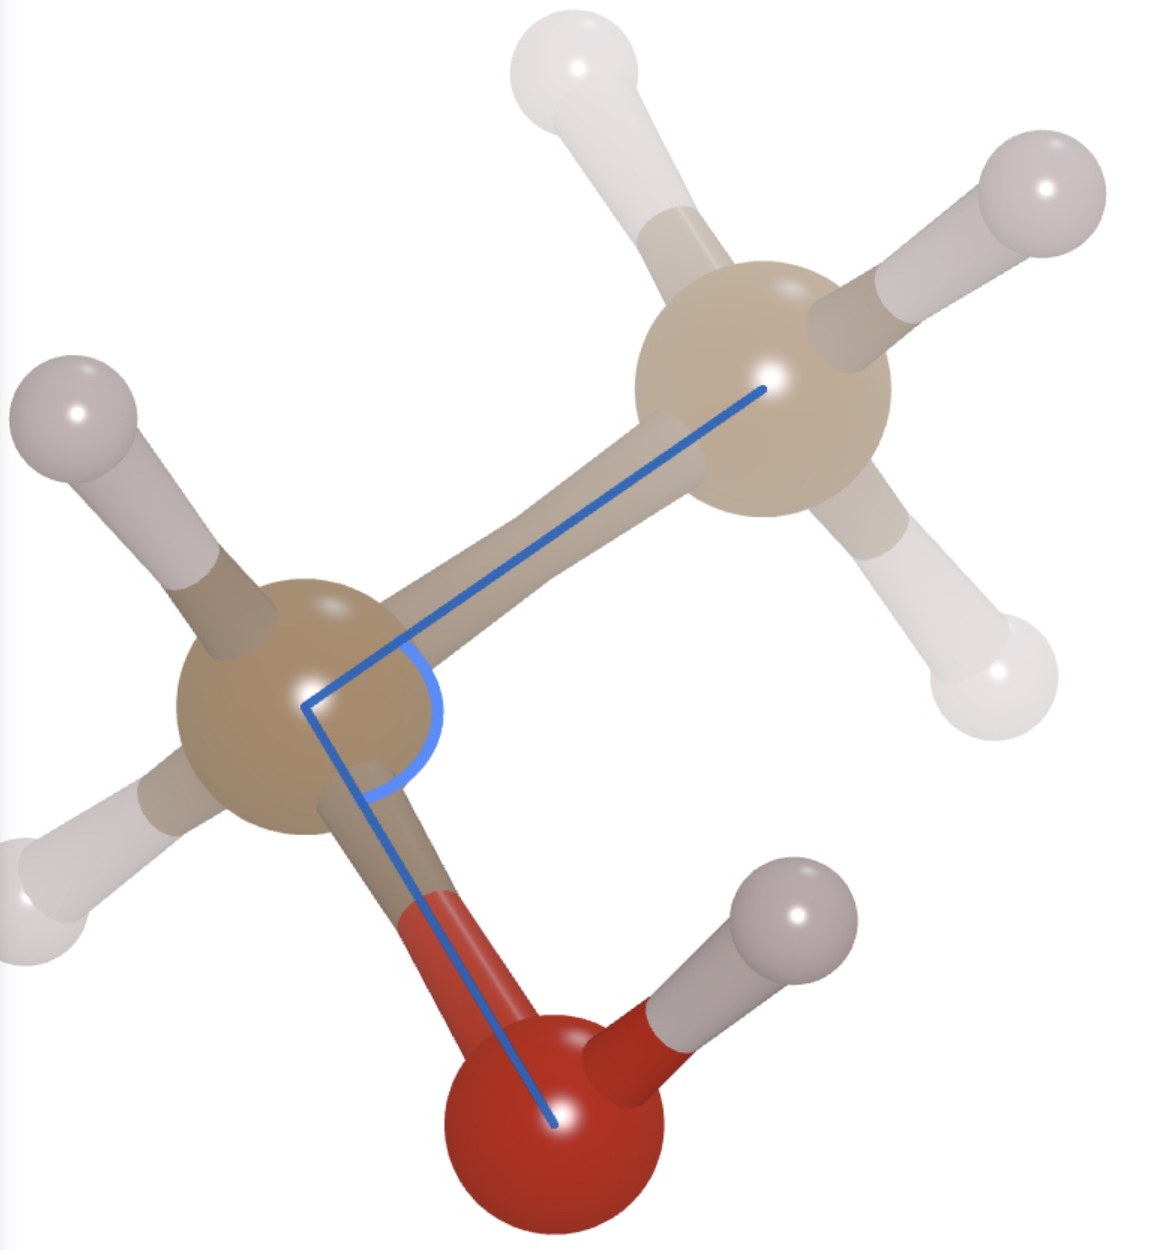
\includegraphics[width=\linewidth]{publication-assets/crop-4185f48c89b2b877f7b1.png}
\end{minipage}
\caption{应用后使用查看器\ui{Bond angle}进行的实际测量。左侧读数为$109.500^\circ$，路径为\#1 C、\#2 C、\#3 O；右侧保留三个重原子和相应角线。本次从\file{ethanol-optimized.json}另载副本，再将该角设为$109.5^\circ$，并非把这一练习值作为优化平衡角。}
\label{fig:ethanol-angle-measured}
\end{figure}


\subsection{整理与优化几何}

\ui{整理几何}使用规则改善明显的局部几何问题；\ui{优化几何}在通用分子模型下进一步调整结构。它们适合准备初始分子，尤其是手工草绘或改动连接之后。优化参数包括最大迭代次数、力收敛容差，以及可选的固定原子序号。

可以先使用默认的最多200次迭代和0.001力容差，预览并应用后，比较结构变化，再测量关注的键长、键角和近距离接触。随书脚本另记录优化方法与收敛过程，便于复核参考结构。后续若要研究精确的平衡几何、构象能量或反应过程，应在计算章节所述的合适方法下继续处理。

随书\file{ethanol-edited.json}保留本例的几何编辑结果，重新导入后测得 C--C 距离 $1.52\,\text{\AA}$、C--C--O 键角 $109.5^\circ$，以原子 9 为末端氢的 C--C--O--H 二面角为 $60^\circ$。\mbox{\file{ethanol-optimized.json}}则经过整理和通用分子模型优化：随书脚本本次用 47 次迭代达到 $0.001\,\mathrm{kJ/(mol\,\text{\AA})}$ 的力阈值。优化允许这些几何量继续改变，因此不能把编辑时指定的数值当作优化后仍然固定的约束。

\subsection{核对分子的组成和几何}\label{sec:molecule-manual-check}

在图形界面中，可以按下面的顺序检查编辑结果，并把前后读数记在一起。

\begin{steps}
  \item 查看结构摘要中的分子式和原子数，与计划建立的分子比较。例如，苯应为$\mathrm{C_6H_6}$，吡啶应为$\mathrm{C_5H_5N}$，乙醇应为$\mathrm{C_2H_6O}$。
  \item 旋转模型，逐个查看发生修改的重原子及其相连的氢。结合已设置的元素、形式电荷、键级与芳香性判断连接是否合理。需要更正时，选中对应原子，使用\ui{原子化学属性}或\ui{设置键级}重新明确设置，再按连接补氢。
  \item 对可疑的短接触，在查看器的\ui{Measurements}中选择\ui{Atom-to-atom distance}并依次点选两个原子；检查键角时选择\ui{Bond angle}并依次点选三个原子。比较修改前后的实际读数，避免只凭球体大小判断原子是否过近。
  \item 保存模型及检查记录。需要查看显式键和原子属性的完整记录时，导出原生JSON；需要逐项诊断数据时，使用完整MATLAB的配套检查脚本。
\end{steps}

\ui{分子诊断}当前检查整个分子。全选后打开命令可以便于核对序号，但局部选择不会把诊断限定到这些原子。完成提示本身不提供“问题已减少”的读数，前后比较应使用组成、连接与测量记录。

% SCREENSHOT: 乙醇键角设置和Bond angle实际读数已由fig:ethanol-angle-parameters及fig:ethanol-angle-measured覆盖；距离/二面角和优化后几何可另补，不要求不存在的详细诊断/优化数据表。

\section{复用建模内容}

完成一个分子后，不必每次从单原子重新开始。先选择连接位点，在顶部\ui{分子建模}页面的同名下拉菜单中打开\ui{片段草绘器}，再选择片段与连接模式，使用窗口中的\ui{连接片段}把片段接到模型。连接前核对片段名称与连接头。用户片段可将经常使用的局部结构保存在库中，重复单元则供高分子构建使用，二者用途不同。

参数对话框中的预设用于保存常用参数。例如，某个超胞变换或表面厚度组合可以保存为有意义的预设，下次加载后再按当前模型调整。预设保存的是参数选择，不代表它会自动适合所有材料。选择集保存的是一组位点，不是该组原子的独立结构副本。

较长的一系列操作可使用\ui{录制}与\ui{保存 Recipe}保留建模过程。对学生作业或团队协作，记录原始结构、操作参数和最终文件，比只保存一张三维截图更容易复查。图像负责说明结构，模型文件负责保留原子和晶胞；两者共同组成一份完整的建模结果。
